% ======================================================================================
% CLUSTERING
%
% graphs to insert:
%	- score vs silhouette coefficient per cluster
%	- sample silhouette values for the best number of clusters
%	- 3D/2D cluster representation for the best number of clusters
% tables to insert:
%	- PCA outcome of the features
%	- object to cluster assignment depending on number of clusters (the best ones)
%	- cluster sizes depending on number of clusters
% figures:
%	- mean values of the features per cluster applied to the object


\section{Clustering}
Here we report the results from clustering depending on different features used.

%\begin{figure}
	%\centering
	%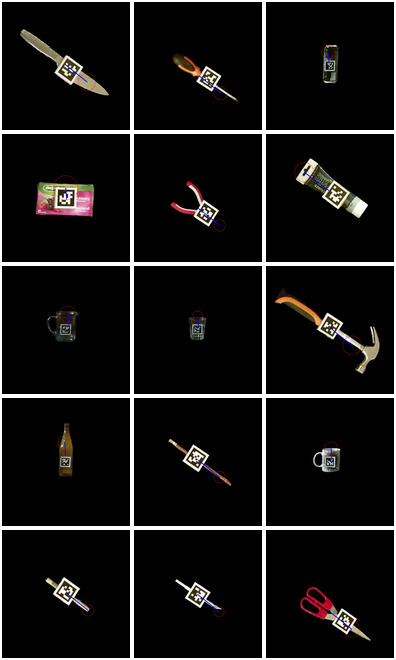
\includegraphics[width=\textwidth]{img/results/object_handovers.jpg}
	%\caption{Resulting handover data applied to each object}
	%\label{fig:object_handovers}
%\end{figure}


\subsection{Principal Component Analysis}


\subsection{K-means}

\begin{figure}
	\begin{subfigure}[b]{\textwidth}
		\input{plot_clustering__mean-silhouette}
		\caption{Mean silhouette coefficient per number of clusters.}
	\end{subfigure}
	\begin{subfigure}[b]{\textwidth}
		\input{plot_clustering__sum-sqr-dist}
		\caption{Sum of squared distances per sample to their closest cluster by number of clusters. Used in the \texttt{elbow method}.}
	\end{subfigure}
	\caption{Mean silhouette coefficient and sum of squared distances per sample to their closest cluster, depending on number of clusters. \texttt{best fit} identifies the possible best number of clusters in accordance to the maximum value of the mean silhouette coefficient and the elbow method.}
\end{figure}

\begin{figure}
	\begin{subfigure}[b]{\textwidth}
		\input{plot_silhouette_5}
		\caption{Silhouette coefficient per samples for five clusters.}
	\end{subfigure}
	\begin{subfigure}[b]{\textwidth}
		\input{plot_silhouette_6}
		\caption{Silhouette coefficient per samples for six clusters.}
	\end{subfigure}
\end{figure}
\begin{figure}
	\ContinuedFloat
	\begin{subfigure}[b]{\textwidth}
		\input{plot_silhouette_7}
		\caption{Silhouette coefficient per samples for seven clusters.}
	\end{subfigure}
	\caption{Silhouette coefficient per sample in each cluster for five, six and seven number of clusters.}
\end{figure}


\begin{figure}
	\begin{subfigure}[b]{\textwidth}
		\input{plot_clustering__clusters-2d}
		\caption{Two-dimensional representation of the samples and their assigned clusters and centroids.}
	\end{subfigure}
	\begin{subfigure}[b]{\textwidth}
		\input{plot_clustering__clusters-3d}
		\caption{Three-dimensional representation of the samples and their assigned clusters and centroids.}
	\end{subfigure}
	\caption{A two-dimensional and three-dimensional representation of the sample space with their assigned clusters and centroids for six clusters.}
\end{figure}


\subsection{Object cluster assignments}

\begin{figure}
	\input{plot_clustering__obj-sampl-assgmnt}
	\caption{}
\end{figure}



% ======================================================================================
% CLASSIFICATION
%
% GRAPHS:
%	- loss per step
%	- accuracy per step (validation and testing)
%	- training speed
% TABLES:
%	- confusion matrix
%	- accuracy per object
%	-

\section{Classification}
Output different results from classification depending on which layers are trained further and network architecture.

\subsection{Initial testing of batch sizes and learning rates}

\subsubsection{Learning rates}

\begin{figure}
	\begin{subfigure}[b]{\textwidth}
		\input{plot_classification__learning-rates__loss}
		\caption{Loss.}
	\end{subfigure}

	\begin{subfigure}[b]{\textwidth}
		\input{plot_classification__learning-rates__val-acc}
		\caption{Validation accuracy.}
	\end{subfigure}
\end{figure}

\begin{figure}
	\ContinuedFloat
	\begin{subfigure}[b]{\textwidth}
		\input{plot_classification__learning-rates__test-acc}
		\caption{Test accuracy.}
	\end{subfigure}
	\caption{Loss, validation and test accuracy for batch size 32 and different learning rates.}
\end{figure}


\subsubsection{Batch sizes}

\begin{figure}
	\begin{subfigure}[b]{\textwidth}
		\input{plot_classification__batch-sizes__loss}
		\caption{Loss.}
	\end{subfigure}

	\begin{subfigure}[b]{\textwidth}
		\input{plot_classification__batch-sizes__val-acc}
		\caption{Validation accuracy.}
	\end{subfigure}
\end{figure}

\begin{figure}
	\ContinuedFloat
	\begin{subfigure}[b]{\textwidth}
		\input{plot_classification__batch-sizes__test-acc}
		\caption{Test accuracy.}
	\end{subfigure}
	\caption{Loss, validation and test accuracy for learning rate 1e-05 and different batch sizes.}
\end{figure}


\subsection{Finetuning parameters}

\subsection{End results}

\begin{figure}
	\input{plot_classification__confmat}
	\caption{Confusion matrix.}
\end{figure}
